% !TEX encoding = UTF-8 Unicode
\chapter{Minecraft in Education}
\section{Einleitung und Motivation}
In unserer heutigen Gesellschaft wird Medienkompetenz immer wichtiger. Sehr viele Berufe benötigen ein hohes Wissen im Bereich von Fachanwendungen (Office, Adobe etc.) für den Computer. 
Aber auch Menschen mit Berufen, ohne den Einsatz von Computern, werden in Ihrer Freizeit und Umgebung immer mehr von der Digitalisierung betroffen.
Smartphones und Tablets sind mittlerweile allgegenwärtig. An den Hochschulen hat fast jeder Student einen Notebook oder ein Tablet.
Bücher werden durch E-Books ersetzt und Vorlesungs-Unterlagen sind nur noch digital verfügbar. Deshalb ist es umso wichtiger, die nächsten Generationen auf diesen Wandel vorzubereiten. 
Ziel muss es sein, den Umgang mit Medien wie Computern von Klein auf zu üben.

Um dies zu erreichen, soll Wissen spielerisch vermitteln und die bisherigen Medien im Schulsystem durch die neue Generation der Lernspiele erweitert werden.
Bisher waren Lernspiele häufig technisch und spielerisch veraltet (im Vergleich zu modernen Computerspielen) und als Einzelspieler-Spiele konzipiert. Moderne Lernspiele setzten hier auf den Online/Mehrspieler-Aspekt um Gruppenarbeit zu fördern und Schulen miteinander zu vernetzen.

Internationale Unternehmen wie Google, Microsoft und Apple haben erkannt wie wichtig diese neue Form der Lernspiele ist und fördern diese im Schulbereich.
Ein Projekt, auf welches in diesem Kapitel näher eingegangen wird, ist Minecraft in Education.

\section{Projekt Minecraft in Education}

Im Jahr 2009 wurde Minecraft (Version old aplha rd-132211) das erste mal vom
Studio Mojang veröffentlicht. Hauptentwickler war Markus Notch Persson. Zu Beginn wurde Minecraft
ausschließlich über die eigene Webseite des Studios vertrieben und löste bereits nach kurzer Zeit,
einen Hype in der Spielwelt aus. 2014 wurde das Studio von Microsoft aufgekauft. Darauf folgte eine Minecraft Version für die mobile Plattformen (Android, IOS) und eine für Windows 10.
\cite{WikiMinecraft}\cite{HeiseMicrosoft}

Minecraft ist ein Computerspiel ohne direktes Spielziel, man spricht von einem \textbf{Sandbox}-Spiel.
Der Spieler übernimmt die Kontrolle über einen Avatar und kann mithilfe von würfelförmigen Blöcken,
in einer 3D-Welt, Konstruktionen erschaffen oder vorhandene bearbeiten. Der Kreativität selbst,
sind dabei kaum Grenzen gesetzt, es gibt eine Vielzahl verschiedener Blockarten mit unterschiedlichen
Eigenschaften. So gibt es Blöcke die physikalisch Korrekt von der Schwerkraft beeinflusst werden,
andere die wiederum in der Luft schweben können und manche die sich wie Flüssigkeiten verhalten.
\cite{WikiMinecraft}

Ein weiterer Grund für die fast unendlichen Möglichkeiten, ist die Erweiterbarkeit des Spiels durch
,von Spielern erstellten, Modifikationen (In der Szene Mods genannt). Mit diesen Erweiterungen ist es
möglich, bis auf das Blocksystem, alle Bereiche des Spieles anzupassen. Einem Weltraumspiel oder einer
Dreidimensionalen Murmelbahn steht nichts im Wege. Neue Arten von Blöcken mit neuen Eigenschaften lassen
sich dabei ebenso einfügen. 

Eine dieser Modifikationen ist das Projekt Minecraft in Education, welches
von Mojang AB und Microsoft Studios gemeinsam entwickelt und Vertrieben wird, mit dem Ziel Minecraft für die Verwendung im Klassenraum anzupassen. \cite{GamepediaMinecraft}

\begin{figure}[ht]
	\centering
	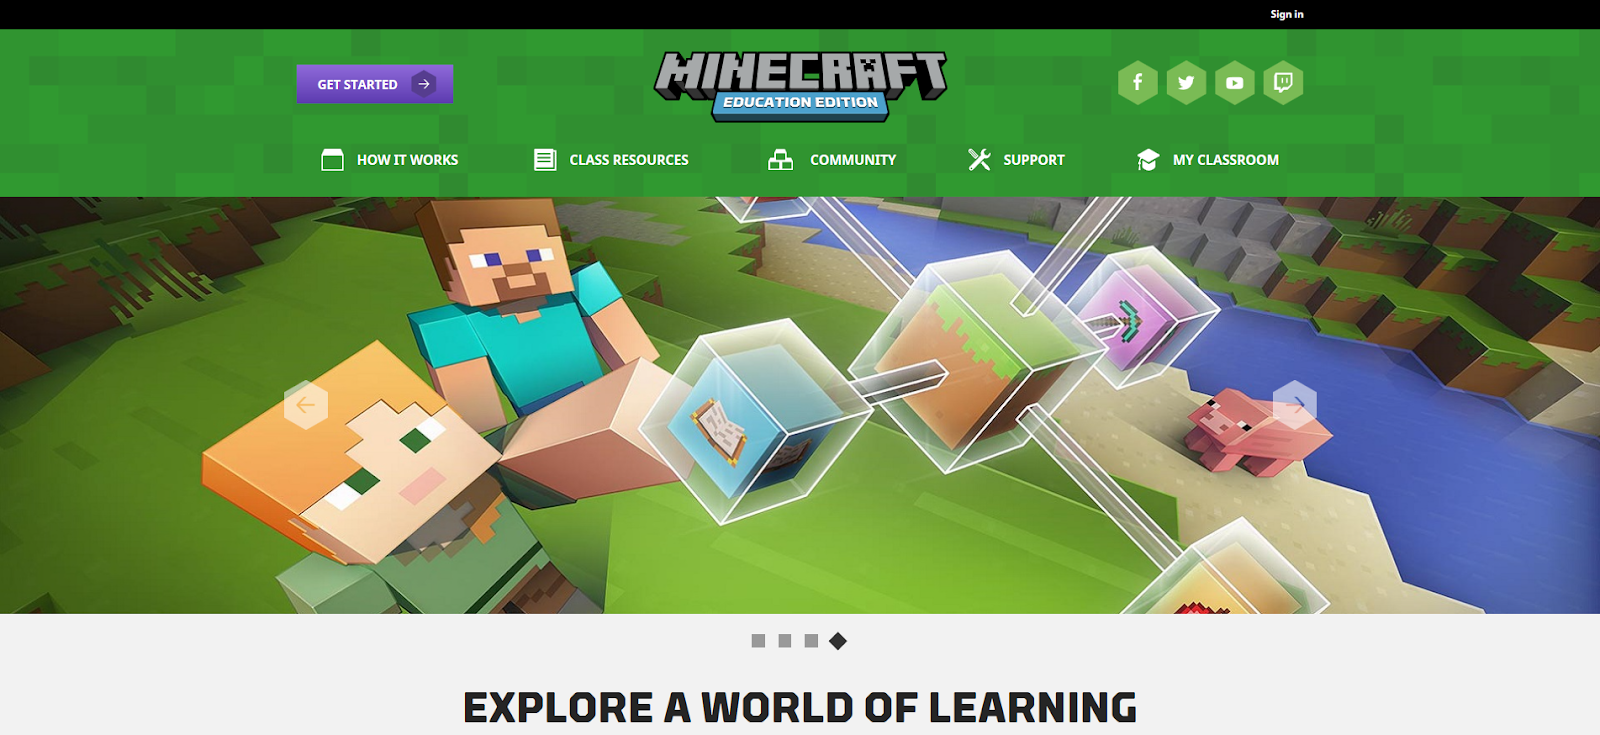
\includegraphics[width=\textwidth,height=\textheight,keepaspectratio]{images/Minecraft.png}
	\caption{Projekt Minecraft in Education \cite{HomepageMinecraftEducation}}
	\label{projectMinecraft}
\end{figure}

Die erste Version wurde am 1.November 2016 veröffentlicht und wird bisher von 2 Millionen Nutzern ausprobiert/genutzt, laut Microsoft.

\section{Aufbau virtueller Klassenraum}
Mit virtuellen Klassenraum ist an dieser Stelle das Treffen der Schüler und Lehrer in einer Spielwelt gemeint.
Innerhalb dieser Welten gibt es viele wichtige Konzepte, die in diesem Abschnitt erläutert werden.
\subsection{Spielwelt}
Die Spielwelt ist der Ort an dem sich die Schüler und Lehrenden treffen um den Unterricht abzuhalten. Jeder Teilnehmer hat zusätzlich eine eigene Spielwelt. Dadurch ist es möglich Gruppenarbeiten durchzuführen, in dem man sich entweder in der Spielwelt der Klasse oder Schülers trifft.

Die Spielwelten können sehr unterschiedliche Formen annehmen. Nachfolgend ist die virtuelle Version des Globe Theatre in London, für den Geschichtsunterricht, abgebildet.

\begin{figure}[ht]
	\centering
	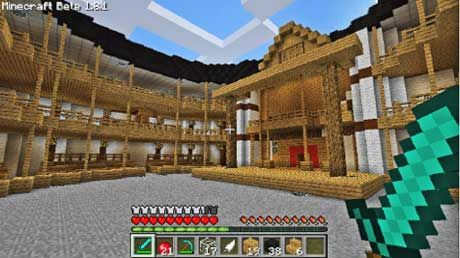
\includegraphics[width=\textwidth,height=\textheight,keepaspectratio]{images/GlobeTheatreLondon.png}
	\caption{Globe Theatre London als virtuelle Version \cite{EdutopiaIdeas}}
	\label{globeTheatreLondon}
\end{figure}

Durch diese virtuellen Schauplätze kann das vermittelte Wissen in Geschichte anschaulich dargestellt werden. Der Schüler erhält dadurch nicht nur die Möglichkeit, Schauplätze zu besuchen, sondern erhält auch Eindrücke wie z.B. die Größe des Kolosseums in Rom. \cite{EdutopiaIdeas}

Diese Information lässt sich mit Worten, Bildern oder Zeichnungen alleine nur schwer vermitteln. Dies ergänzt somit sinnvoll die eingesetzten Medien im Unterricht.

\subsection{Kameras}
Kameras sind Objekte, die ein Spieler mit sich führt. Sie werden verwendet um den Lernfortschritt oder Entdeckungen festzuhalten. Dies ist sehr wichtig, da nicht nur der Spaß am Spielen im Vordergrund steht, sondern auch die Überprüfbarkeit der Leistung durch den Lehrer. Nach dem Unterricht, kann so zu einem beliebigen Zeitpunkt, das Ergebnis eines Schülers betrachtet und bewertet werden.

\subsection{Blöcke}
Eine Spielwelt besteht aus Blöcken mit unterschiedlichen Eigenschaften. Diese können unter anderem verwendet werden um die Spielwelt zu begrenzten, Flüssigkeiten darzustellen oder Gravitation zu simulieren.

Mit dem \textbf{Redstone}-Block können beispielsweise elektrische Schaltungen entworfen werden. Dazu nimmt der Schüler mehrere Blöcke und verknüpft sie miteinander. Über einen Schalter werden diese anschließend unter Strom gesetzt und das Ergebnis wird sichtbar, wie nachfolgend dargestellt.

\begin{figure}[ht]
	\centering
	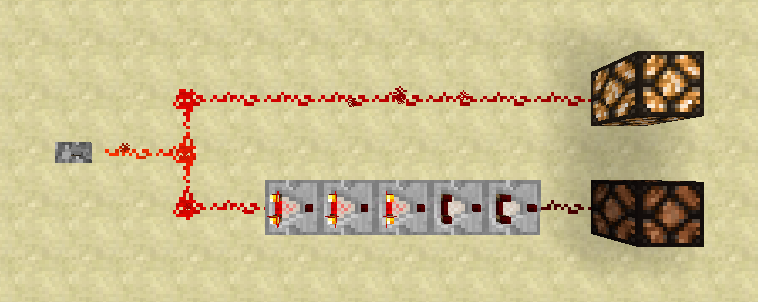
\includegraphics[width=\textwidth,height=\textheight,keepaspectratio]{images/RedstoneSignalverzoegerer.png}
	\caption{Signalverzögerer mit \textbf{Redstone} \cite{GamepediaMinecraft}}
	\label{redstoneSignalDelay}
\end{figure}

Die dargestellte Schaltung verzögert ein Signal. Das \textbf{Redstone} sind die roten Linien, welche unter Storm gesetzt werden. Der etwas hellere Block oben rechts, stellt eine Lampe dar, die leuchtet. Unten auf der rechten Seite befindet sich eine Lampe, die noch aus ist und verzögert angeschaltet wird.
Dies ist nur ein mögliches Szenario, mit \textbf{Redstone} lassen sich beliebige Schaltungen simulieren.
Dadurch kann dem Schüler wissen im Bereich Technik, Physik und auch Programmieren vermitteln.

Damit die Schüler nicht alle Bereiche der Spielwelt verändern können und um Chaos zu verhindern, kann der Lehrende die sogenannten \textbf{Deny} und \textbf{Allow}-Blöcke verwenden. Mit einem Allow-Block, wird ein bestimmtes Gebiet zum Bearbeiten freigegeben, mit dem Deny-Block hingegen verboten. Dies ist wichtig um den Schülern Grenzen festzulegen.
Die folgenden Abbildung zeigt einen Allow (Hellbraun) und Deny (Grau)-Block.

\begin{figure}[ht]
	\centering
	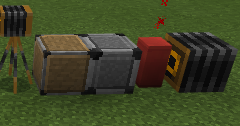
\includegraphics{images/AllowAndDenyBlocks.png}
	\caption{Allow und Deny Blöcke \cite{GamepediaMinecraft}}
	\label{allowDenyBlocks}
\end{figure}

\subsection{NPCs}
Ein wichtiges Element im virtuellen Klassenraum sind die sogenannten NPCs (Non-player characters).
Darunter versteht man Figuren, in der virtuellen Welt, die nicht selbst vom Lehrer gesteuert werden und Verwendung finden, um dem Spieler Anleitung oder Hinweise zu geben. Dadurch kann ein Lehrer wichtige Anmerkungen für die Schüler geben, die zu jedem Zeitpunkt abgerufen werden können, der Lehrer selbst muss nicht anwesend sein.
Dies kann eingesetzt werden, um noch einmal eine Zusammenfassung des Unterrichtstoffes zu geben oder die Aufgabenstellung zu wiederholen. Nachfolgend zeigt, wie ein NPC in Minecraft aussehen kann.

\begin{figure}[ht]
	\centering
	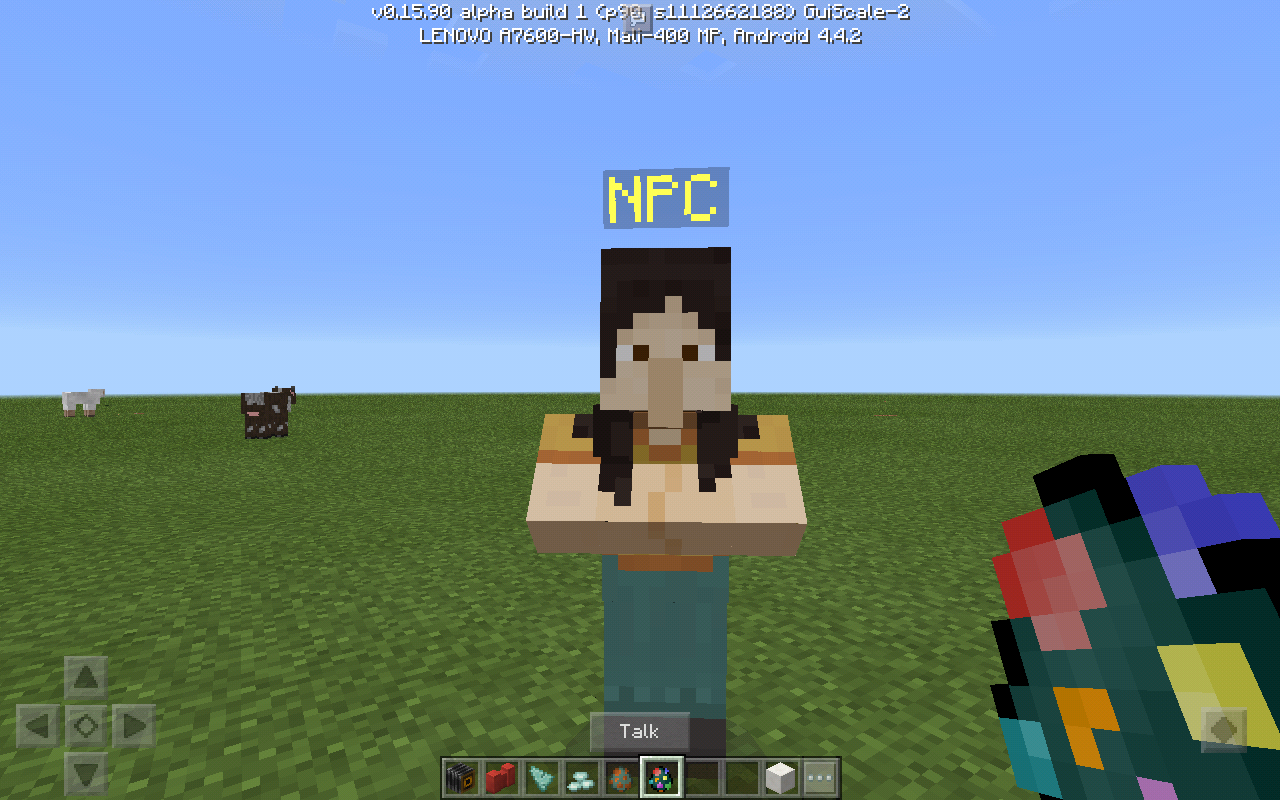
\includegraphics[width=\textwidth,height=\textheight,keepaspectratio]{images/NPC.png}
	\caption{Ein NPC \cite{GamepediaMinecraft}}
	\label{npc}
\end{figure}

- Programmieren lernen
- Physik/Mathematisch praktisch nachvollziehen
- VR Unterstützung für mehr 

\section{Vernetzung von Schulen}
- Tutoren
- Wissen verteilt
- Unterstützt den Fachkräftemangel abzuschwächen

- Geteilte Unterrichtspläne
\section{Auswirkungen auf das Lernverhalten?}
- Motivation durch Spaß
- Spielerisch Wissen erlangen
- Gruppenarbeit -> Teamfähigkeit!

\section{Gibt es Risiken?}
- Überforderung von Schülern
- Diese Art des Lernens eignet sich nicht für alle Schüler
- Anonymität des Internets, Kommunikation sehr direkt

\section{Erfahrungsberichte}

\section{Fazit}
- Keine neue Lernmethode
- Verbesserte Methode
- Koordination und Lernbereitschaft steigt, durch Spaß am Probieren
- Für viele Fächer geeignet
- Wie alle Medien sollte es unterstützend und nicht als einziges Medium eingesetzt werden